\section{Introduction}\label{introduct}
A well-studied phenomenon in material science concerns the coarsening of microstructure found in metals, porcelains, and other common materials.  Typically, these materials have polycrystalline structure, where each grain has a particular orientation.  Annealing induces an evolution on grain boundaries which reduces their total length.  During this process, grains are deleted (and not created), causing coarsening of microstructure through an increase of average grain area (see Fig. \ref{samplegrains}).  Microstructure can determine material properties. For instance, the Hall-Petch effect gives a relation between yield stress and average grain size (see \cite{anderson2005fracture}, section 5.2.3).     More scientific and  mathematical properties of grain networks can be found in \cite{fradkov1994two,thompson2001grain}.


 
 
Grain coarsening in two dimensions  can be modeled by a geometric network, or planar graph $G(t) \subset \mathbb{R}^2$, $t\in (0,T)$, with edges  that evolve in time. Faces of $G$ are called \textbf{grains}, and edges are referred to as \textbf{boundaries}. An idealization of the coarsening process assumes that grain boundaries are isotropic, or that grain boundary energies are identical along edges of the network. Under this idealization, we  define a \textbf{grain network with existence interval} $(0,T)$  as a geometric finite planar graph $G(t)$ which satisfies the
following restrictions for all $t\in(0,T)$:



\begin{enumerate}
\item (\textbf{Herring's Condition})   $G(t)$ is trivalent, and angles between two edges at a vertex are fixed at 120 degrees.
This restriction follows from a force balance law on edges  emanating from a vertex (see \cite{herring1999surface}).\item (\textbf{Mean Curvature Flow}) Boundaries are smooth, and satisfy mean curvature flow.  This means that the time evolution of a smooth boundary $\gamma(x,t)\subset \mathbb R^2$ is also smooth, and satisfies 
 \begin{equation} \label{curveflow}
\partial_t \gamma(x,t) = M\sigma \kappa(x,t)  \vec n(x,t), \quad t\in(0,T), x \in \mathbb{R}^2,
\end{equation}
with $M$ and $\sigma$ denoting grain mobility and surface energy constants, $\vec n(x,t)$ denoting the inward unit normal, and $\kappa(x,t)$ denoting mean curvature. This type of motion was observed experimentally by Beck for crystallites in metals \cite{bec52}.
\end{enumerate}
     


Note that grain networks retain their topological structure during their existence time.  The parabolic PDE (\ref{curveflow})  is referred to as curve-shortening flow, and it can in fact be shown that the total edge length of a network decreases in time \cite{barmak2011entropy}. A theorem of curve shortening flow on grain networks, due to von Neumann and Mullins \cite{mul56,von1952discussion} gives an elegant relation between a topological quantity (sides of a grain) and a geometrical quantity (area of a grain).

\begin{figure}
\includegraphics[width=\textwidth]{samplegrains.png}
\caption{\textbf{Coarsening of a grain network.} Grains in material microstructure delete through annealing, causing the average grain size to increase.}\label{samplegrains}
\end{figure}
 


\begin{theorem}(\textbf{The von Neumann-Mullins $n-6$ rule}). For a grain with area $A$ and $n$ sides,
\begin{equation}
\frac{dA}{dt} = M\sigma\frac \pi 3 (n-6).
\end{equation}  
\end{theorem}
One consequence of the $n-6$ rule  is  that grains with less than six sides may shrink to a point in finite time. Such deletions, along with possible edge deletions, result in networks with vertices that violate Herring's condition.  This raises the question: What types of solutions exist with initial conditions that are not grain networks?  Specifically, the \textbf{continuation problem for a planar network $G$} asks the following: If we are given a planar network $G$ with vertices that may not satisfy Herring's conditions,  is there an  $\varepsilon>0$ where $G(t)$ is a grain network for $t\in (0, \varepsilon)$, and $G(t)\rightarrow G$ in the Hausdorff distance as $t\rightarrow  0^+$? Another interesting question is whether the flow is unique, or if it can become unique under additional assumptions.

Currently, there are no comprehensive answers to the above questions.  Viewed as a problem in parabolic PDE theory, the current focus is local, fixing on simplified models with initial conditions of $k$ rays meeting at a vertex. Schnurer and Shulze found a unique self-similar solution with initial conditions of three rays meeting at arbitrary angles \cite{sch07}.  Mazzeo and Saez  generalized with the $k$-ray initial conditions, and discovered a bijection between self-similar solutions   and $k$-Steiner trees of a hyperbolic metric \cite{maz07}.  On the computational front, techniques of flowing through a graph not satisfying the grain network conditions include level set \cite{elsey2009diffusion}  and variational \cite{kin06} methods. 
 




\section{Mean-field models of grain growth}\label{fradkov}
Another approach to studying grain boundary coarsening involves using mean field assumptions to gather bulk statistics of grain behavior.  A well known kinetic model is due to Fradkov \cite{fra882,fra881}, who exploits  the $n-6$ rule, along with an additional deterministic rule for side redistribution, to derive kinetic equations for densities of grains with a specific number of sides.   Fradkov makes the following mean field assumptions about the redistribution of sides when either a grain or edge deletes:
\begin{enumerate}
\item If a grain or side deletes, topological changes of grains will be selected in proportion to the number of sides of grains, and independent of their areas.  For instance, if a singular event causes a grain to lose a side, the probability that a particular grain with $j$ sides will drop to one with $j-1$ sides is
\begin{equation}
p_j=\frac{j}{\sum_{k>1} kN_k},
\end{equation}
where $N_k$ is the number of grains with $k$ sides.  
  This eliminates the notion of grains having neighbors.  
\item A free parameter $\beta$ is introduced which is defined as the constant ratio between side deletions and grain deletions.  Such an assumption comes from the lack of a topological rule for edge growth.  
\end{enumerate}

For a number density $f_n(a,t)$ of $n $ sided grains with area $a$ at time $t$, the Fradkov equations take the form of a transport equation with a topological source term:
\begin{equation}
\partial_t f_n(a,t)+(n-6)\partial_a f_n(a,t) = \Gamma(f(t))(Jf)_n(a,t) \quad (a,t) \in (0,\infty)^2, n \ge 2 ,
\end{equation}
with a collision operator $J$ and coupling weight $\Gamma$ determined from conservation of area and polyhedral defect (networks retain an average of six sides). Well-posedness and self-similar solutions for the Fradkov model can be found in \cite{henseler2008kinetic, her12}.



 
\section{PDMPs and grain coarsening}\label{pdmpgraincoarse}
The main goal of this thesis is to understand grain  statistics as a hydrodynamic limit of finitely many grains respecting deterministic drift and random topological transitions.  In particular, we will  construct limiting kinetic equations describing the evolution of grain area densities for the class of grains with a fixed number of sides.   Toward this goal, the main tool we use is the theory of piecewise deterministic Markov process (PDMP).  The construction and theory of PDMPs will be discussed in Chapter 2.  However, not much is lost to think of a PDMP  as a generalization of a jump process for particles that drift on vector fields.    

For the problem of grain coarsening, we wish to build a PDMP $X(t)$ that tracks a finite set of grains $(g_1,\dots, g_n) =  ((a_1,s_1), \dots, (a_n,s_n))$ with areas $a_i>0$ and side numbers $s_i \in \mathbb N.$  
Note that the dimension of $X(t)$ can change with time, as grains delete from coarsening. Grain areas change at a constant rate, following the $n-6$ rule until a grain shrinks to a point, or an edge deletes (we will make an assumption on side deletion rates based on total particle number).  At that time, we impose mean field assumptions to change topologies of grains. 

 

 
\begin{figure}  
\begin{centering} 
 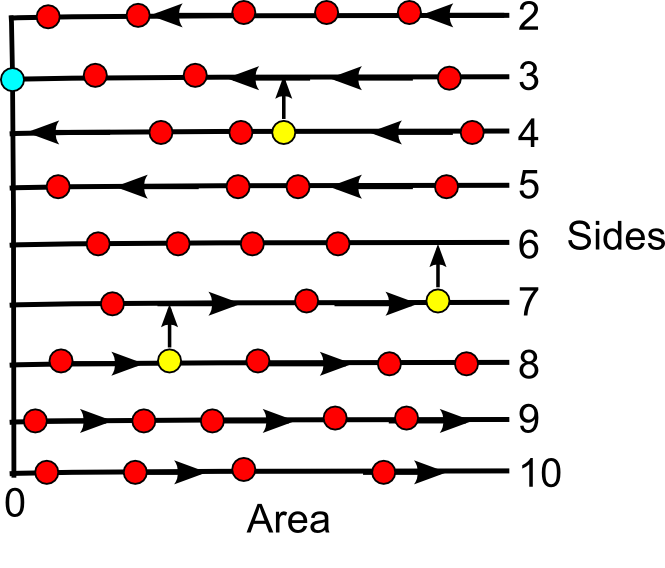
\includegraphics[width = .4\textwidth]{graintops.png} 
 \caption{\textbf{Grain growth via a PDMP}. Particles drift according to their number of sides. Each tier denotes particles of different side numbers. In this instance, a vanishing grain in tier three triggers a  random reassignment  of the number of sides of grains in tiers 4,7, and 8.}
\end{centering}
\end{figure}

\section{Overview}
 
In Chapter 2, we describe a PDMP in generality. We then state its infinitesimal generator $\mathcal A$, and the class of functionals $\mathcal D(\mathcal A)$ that give rise to martingales through the Dynkin formula.    

In Chapter 3, we  study a simplified version of the PDMP described in Section \ref{pdmpgraincoarse}. Here, particles drift on the positive half-line until reaching the origin, where they are reassigned according to a probability density $p(x)$.     We first prove that for empirical densities approaching nonatomic initial conditions, the densities $u(x,t)$ of particles converge to a weak form of the limiting kinetic equation
\begin{alignat}{2}\label{pde1}  
\partial_tu(x,t) - \partial_x u(x,t) = p(x)u(0,t) \quad t, x \in \mathbb{R}^+, \\
u(x,0) = u_0(x) . \nonumber
\end{alignat}
We then focus on constructing measure valued weak solutions of (\ref{pde1}) with mild restrictions on initial data. Finally, we use a popular result of renewal theory to show the existence of an attractor under certain assumptions.

  Chapter 4 is a generalization of PDMPs on grain networks described in Section \ref{pdmpgraincoarse}.  Here, we show the existence of fluid limits of PDMPs that allow generalized rules and probability distributions for particle jumps between different species.  As in Chapter 3, we will show the existence of a weak limit for densities $u_k(x,t)$ on $L_k$, that satisfy the advection-reaction equations
\begin{eqnarray} \label{pde2}
  \lefteqn{\partial_t u_k(x,t)+\partial_{x}(v_k(x)u_{k}(x,t))=  \phantom{u_j(x,t)\mathbf{1}_{R^{(l)}_{ij}}
-K^{(l)}W_k^{(l)}(t)u_k(x,t)}}\label{smoooth}\\
 && \sum_{l = 1}^{M_-}u_l(0,t)v_{l}(0)\left[\sum_{i = 1}^{M}\sum_{j= 1}^{K^{(l)}} W_i^{(l)}(t)u_i(x,t)\mathbf{1}_{R^{(l)}_{ij}=k}
-K^{(l)}W_k^{(l)}(t)u_k(x,t)\right]\nonumber\\ 
&&+\frac{\beta G(t)}{G^{int}(t)}\left( \sum_{i = 1}^{M}\sum_{j= 1}^{K^{int}} w^{int} _iu_{i}(x,t)\mathbf{1}_{R^{int}_{ij} = k}-K^{int}w^{int}_ku_{k}(x,t)
 \right), \nonumber
 \end{eqnarray}
 with initial conditions
 \begin{equation}
u_k(x,0) = u_{k}^0(x), \quad k = 1,\dots, M. \nonumber
\end{equation}
The solutions of (\ref{pde2}) will be shown to be unique in the class of $L^1\cap L^\infty(\mathbb R^+)$ functions.

Finally, in Chapter 5, we return to the problem of grain coarsening. First, we examine the topological behavior of grain networks before and after a grain or side vanishes. After finding a finite set of rules that dictate topological changes,    we then define the various free parameters in the $k$-species model to align with a mean field model for grain coarsening.  Next, we prove some basic properties of the limiting kinetic equation, such as conservation of mass and polyhedral defect.  Finally, we end the chapter with a computational investigation of grain growth, and raise several conjectures about grain statistics.   
  

